\documentclass[tikz,border=12pt]{standalone}
\usepackage[T1]{fontenc}
\usepackage{mathpazo}
\usepackage{amsmath,amssymb}
\usetikzlibrary{arrows.meta, positioning, calc, decorations.pathreplacing}

\definecolor{stblue}{HTML}{7B97AD}
\definecolor{rwgold}{HTML}{B8995E}
\definecolor{sage}{HTML}{7A9A7E}
\definecolor{dkbrown}{HTML}{3D3530}
\definecolor{wmgray}{HTML}{7B7067}
\definecolor{cream}{HTML}{F9F6F0}
\definecolor{border}{HTML}{D4C9B8}
\definecolor{terracotta}{HTML}{C47A6A}
\definecolor{lavender}{HTML}{907EA0}

\begin{document}
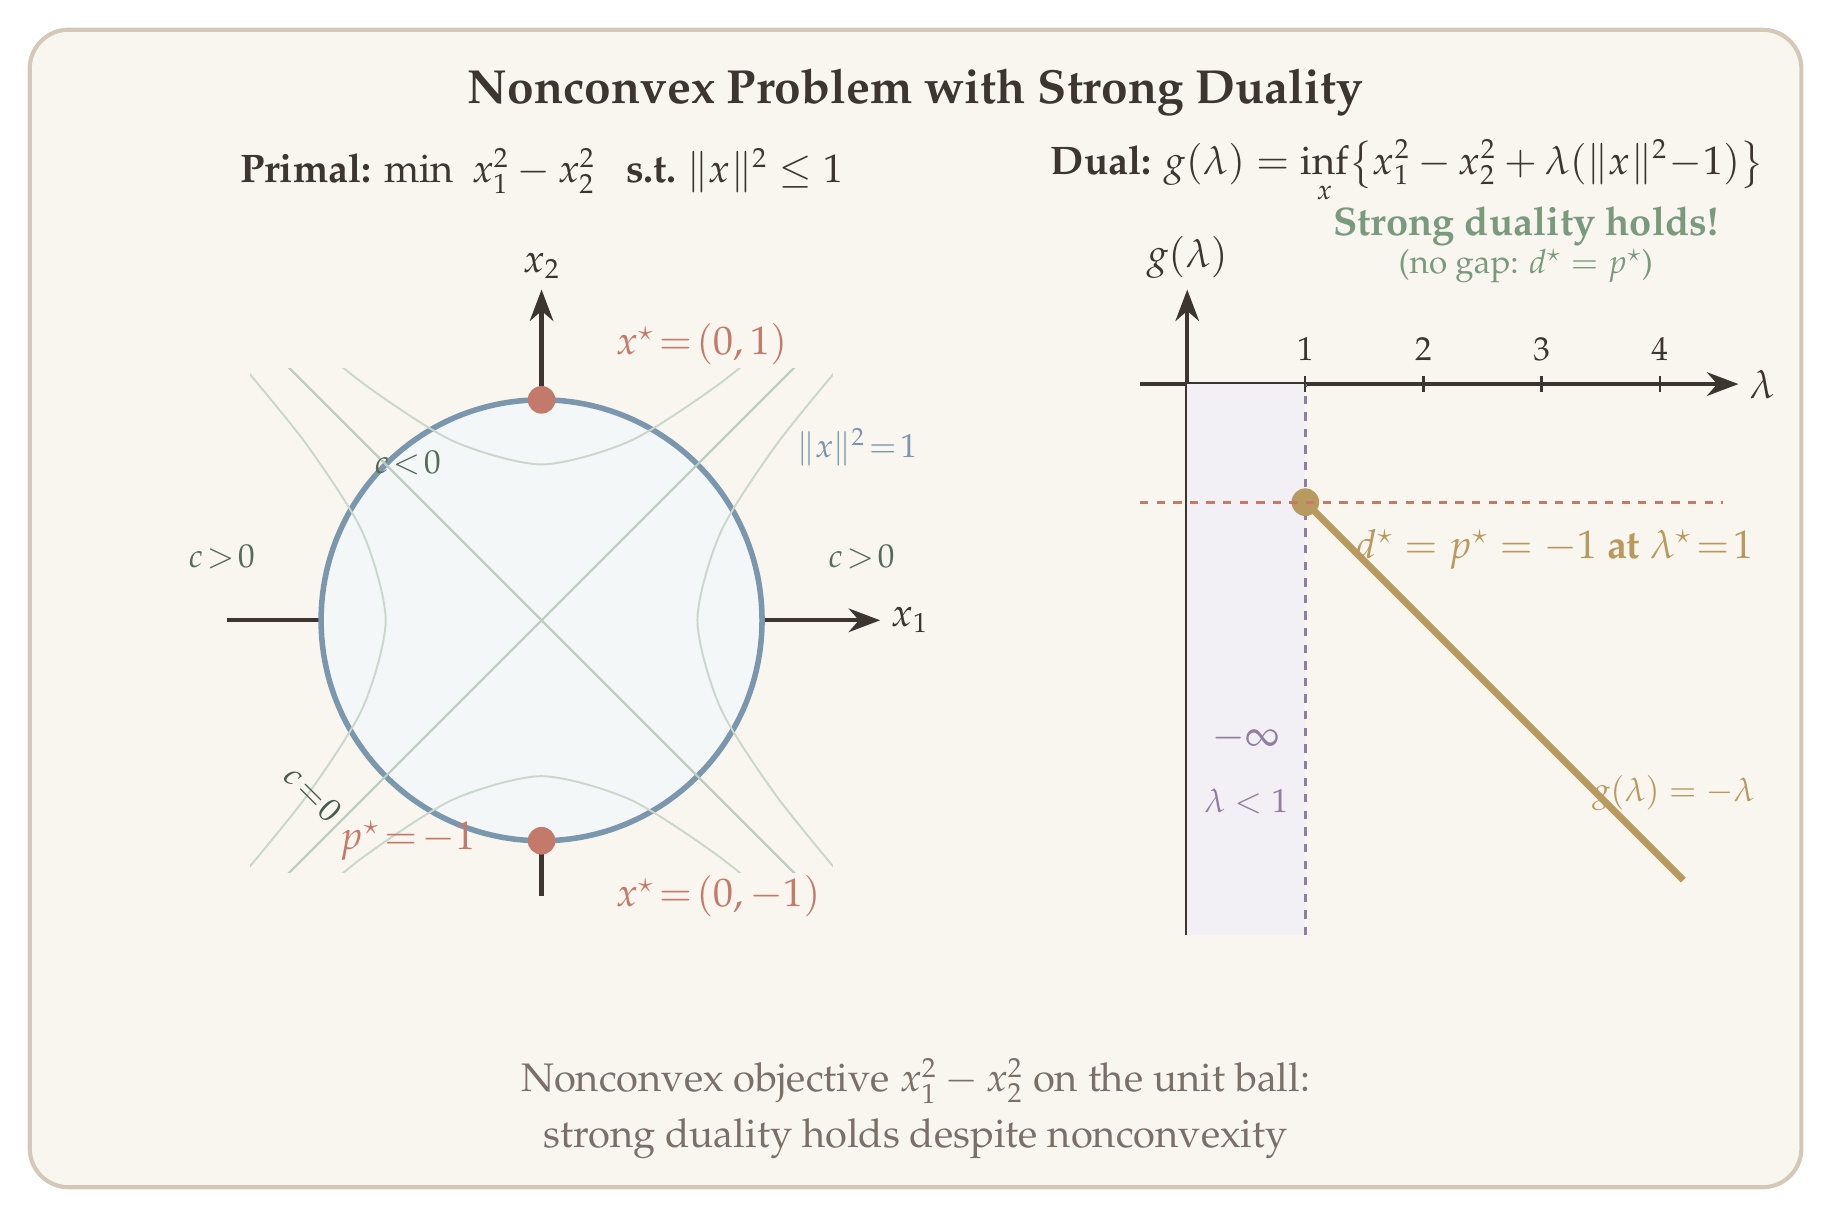
\begin{tikzpicture}[>={Stealth[length=4mm, width=3mm]}, line width=1.5pt]

% Background
\fill[cream, rounded corners=14pt] (-2,-4.2) rectangle (20.5,10.5);
\draw[border, line width=1.5pt, rounded corners=14pt] (-2,-4.2) rectangle (20.5,10.5);

% Title
\node[font=\LARGE\bfseries, text=dkbrown, align=center] at (9.25,9.7)
  {Nonconvex Problem with Strong Duality};

% ================================================================
% LEFT PANEL: Primal -- min x1^2 - x2^2  s.t.  x1^2 + x2^2 <= 1
% ================================================================
\begin{scope}[shift={(0,0)}]

% Panel label — well above the plot
\node[font=\Large\bfseries, text=dkbrown, align=center] at (4.5,8.7)
  {Primal: $\min\; x_1^2 - x_2^2$ \; s.t.\ $\|x\|^2 \le 1$};

% Center of the circle at (4.5, 3.0), radius = 2.8 tikz units
% Maps: real (x1,x2) -> tikz (4.5 + 2.8*x1, 3.0 + 2.8*x2)

% Axes
\draw[->, dkbrown, line width=1.5pt] (0.5,3.0) -- (8.8,3.0)
  node[right, font=\Large, text=dkbrown] {$x_1$};
\draw[->, dkbrown, line width=1.5pt] (4.5,-0.5) -- (4.5,7.2)
  node[above, font=\Large, text=dkbrown] {$x_2$};

% Unit circle (constraint) — filled then stroked
\fill[stblue!8] (4.5,3.0) circle (2.8);
\draw[stblue, line width=2pt] (4.5,3.0) circle (2.8);
\node[font=\large, text=stblue, anchor=west] at (7.6,5.2) {$\|x\|^2\!=\!1$};

% Contour lines of f = x1^2 - x2^2 (hyperbolas), clipped to a region
\begin{scope}
\clip (0.8,-0.2) rectangle (8.2,6.2);

% c = 0 contour: x1 = +- x2, the diagonals through center
\draw[sage!50, line width=0.8pt] (4.5-3.5, 3.0+3.5) -- (4.5+3.5, 3.0-3.5);
\draw[sage!50, line width=0.8pt] (4.5-3.5, 3.0-3.5) -- (4.5+3.5, 3.0+3.5);

% c = -0.5: x2^2 - x1^2 = 0.5 -> upper/lower branches opening along x2
\draw[sage!40, line width=0.7pt] plot[smooth, tension=0.45] coordinates {
  ({4.5-1.2*2.8}, {3.0+sqrt(1.44+0.5)*2.8})
  ({4.5-0.8*2.8}, {3.0+sqrt(0.64+0.5)*2.8})
  ({4.5-0.4*2.8}, {3.0+sqrt(0.16+0.5)*2.8})
  ({4.5},         {3.0+0.707*2.8})
  ({4.5+0.4*2.8}, {3.0+sqrt(0.16+0.5)*2.8})
  ({4.5+0.8*2.8}, {3.0+sqrt(0.64+0.5)*2.8})
  ({4.5+1.2*2.8}, {3.0+sqrt(1.44+0.5)*2.8})
};
\draw[sage!40, line width=0.7pt] plot[smooth, tension=0.45] coordinates {
  ({4.5-1.2*2.8}, {3.0-sqrt(1.44+0.5)*2.8})
  ({4.5-0.8*2.8}, {3.0-sqrt(0.64+0.5)*2.8})
  ({4.5-0.4*2.8}, {3.0-sqrt(0.16+0.5)*2.8})
  ({4.5},         {3.0-0.707*2.8})
  ({4.5+0.4*2.8}, {3.0-sqrt(0.16+0.5)*2.8})
  ({4.5+0.8*2.8}, {3.0-sqrt(0.64+0.5)*2.8})
  ({4.5+1.2*2.8}, {3.0-sqrt(1.44+0.5)*2.8})
};

% c = 0.5: x1^2 - x2^2 = 0.5 -> left/right branches opening along x1
\draw[sage!40, line width=0.7pt] plot[smooth, tension=0.45] coordinates {
  ({4.5+sqrt(1.44+0.5)*2.8}, {3.0-1.2*2.8})
  ({4.5+sqrt(0.64+0.5)*2.8}, {3.0-0.8*2.8})
  ({4.5+sqrt(0.16+0.5)*2.8}, {3.0-0.4*2.8})
  ({4.5+0.707*2.8},          {3.0})
  ({4.5+sqrt(0.16+0.5)*2.8}, {3.0+0.4*2.8})
  ({4.5+sqrt(0.64+0.5)*2.8}, {3.0+0.8*2.8})
  ({4.5+sqrt(1.44+0.5)*2.8}, {3.0+1.2*2.8})
};
\draw[sage!40, line width=0.7pt] plot[smooth, tension=0.45] coordinates {
  ({4.5-sqrt(1.44+0.5)*2.8}, {3.0-1.2*2.8})
  ({4.5-sqrt(0.64+0.5)*2.8}, {3.0-0.8*2.8})
  ({4.5-sqrt(0.16+0.5)*2.8}, {3.0-0.4*2.8})
  ({4.5-0.707*2.8},          {3.0})
  ({4.5-sqrt(0.16+0.5)*2.8}, {3.0+0.4*2.8})
  ({4.5-sqrt(0.64+0.5)*2.8}, {3.0+0.8*2.8})
  ({4.5-sqrt(1.44+0.5)*2.8}, {3.0+1.2*2.8})
};

\end{scope}

% Contour labels — larger, well-spaced away from optimal points and each other
\node[font=\large, text=sage!70!black, anchor=west] at (8.0,3.8) {$c\!>\!0$};
\node[font=\large, text=sage!70!black, anchor=east] at (1.0,3.8) {$c\!>\!0$};
\node[font=\large, text=sage!60!black, rotate=-45] at (1.6,0.8) {$c\!=\!0$};

% Mark optimal points x* = (0, +-1) at tikz (4.5, 5.8) and (4.5, 0.2)
\fill[terracotta] (4.5,5.8) circle (5pt);
\fill[terracotta] (4.5,0.2) circle (5pt);

% Labels for optimal points — offset further from the dots
\node[font=\Large\bfseries, text=terracotta, anchor=south west] at (5.3,6.1)
  {$x^\star\!=\!(0,1)$};
\node[font=\Large\bfseries, text=terracotta, anchor=north west] at (5.3,-0.1)
  {$x^\star\!=\!(0,-1)$};

% c < 0 label placed between the two optimal points (inside circle)
\node[font=\large, text=sage!70!black] at (2.8,5.0) {$c\!<\!0$};

\node[font=\Large\bfseries, text=terracotta, anchor=east] at (3.8,0.2) {$p^\star\!=\!-1$};

\end{scope}

% ================================================================
% RIGHT PANEL: Dual  g(lambda) for lambda >= 0
% ================================================================
\begin{scope}[shift={(11.5,0)}]

% Panel label
\node[font=\Large\bfseries, text=dkbrown, align=center] at (4,8.7)
  {Dual: $g(\lambda) = \displaystyle\inf_{x}\bigl\{x_1^2 - x_2^2 + \lambda(\|x\|^2\!-\!1)\bigr\}$};

% g(lambda) = inf_x { (1+lambda)*x1^2 + (lambda-1)*x2^2 } - lambda
% lambda >= 1: both coefficients >= 0, so inf = 0, g(lambda) = -lambda.
% 0 <= lambda < 1: coefficient of x2^2 is negative, so inf = -infty.

% Axes
% lambda in [0, 5] -> tikzX, with lambda=0 at tikzX=1.2, scale 1.5 per unit
%   tikzX = 1.2 + 1.5*lambda
%   lambda=1 -> 2.7,  lambda=2 -> 4.2,  lambda=3 -> 5.7,  lambda=4 -> 7.2
% g-axis: g=0 at tikzY=6.0, scale 1.5 per unit downward (more spread)
%   tikzY = 6.0 + 1.5*g
%   g=-1 -> 4.5,  g=-2 -> 3.0,  g=-3 -> 1.5,  g=-4 -> 0.0,  g=-5 -> -1.5

\draw[->, dkbrown, line width=1.5pt] (0.6,6.0) -- (8.2,6.0)
  node[right, font=\Large, text=dkbrown] {$\lambda$};
\draw[->, dkbrown, line width=1.5pt] (1.2,-1.0) -- (1.2,7.2)
  node[above, font=\Large, text=dkbrown] {$g(\lambda)$};

% Region lambda < 1: g = -infty (shaded)
% lambda=1 -> tikzX = 2.7
\fill[lavender!12] (1.2,-1.0) rectangle (2.7,6.0);
\draw[lavender, dashed, line width=1pt] (2.7,-1.0) -- (2.7,6.0);
\node[font=\Large\bfseries, text=lavender] at (1.95,1.5) {$-\infty$};
\node[font=\large, text=lavender] at (1.95,0.7) {$\lambda<1$};

% g(lambda) = -lambda for lambda >= 1
% lambda=1: g=-1 -> tikz (2.7, 4.5)
% lambda=2: g=-2 -> tikz (4.2, 3.0)
% lambda=3: g=-3 -> tikz (5.7, 1.5)
% lambda=4: g=-4 -> tikz (7.2, 0.0)
\draw[rwgold, line width=2.5pt] (2.7,4.5) -- (7.5,-0.3);

% Mark d* = p* = -1 at lambda* = 1
\fill[rwgold] (2.7,4.5) circle (5pt);

% p* = d* dashed reference line at g=-1 -> tikzY=4.5
\draw[terracotta, dashed, line width=1pt] (0.6,4.5) -- (8.0,4.5);

% Combined label: placed to the right with enough space below lambda axis
\node[font=\Large\bfseries, text=rwgold, anchor=west] at (3.2,3.9)
  {$d^\star = p^\star = -1$ at $\lambda^\star\!=\!1$};

% Strong duality callout — placed above the axis, well clear
\node[font=\Large\bfseries, text=sage, align=center] at (5.5,8.0)
  {Strong duality holds!};
\node[font=\large, text=sage, align=center] at (5.5,7.5)
  {(no gap: $d^\star = p^\star$)};

% g(lambda) label on the ray
\node[font=\large, text=rwgold, anchor=west] at (6.2,0.8) {$g(\lambda)=-\lambda$};

% Tick marks on lambda axis — placed above
\draw[dkbrown, line width=0.8pt] (2.7,5.9) -- (2.7,6.1);
\node[font=\large, text=dkbrown, above] at (2.7,6.15) {$1$};
\draw[dkbrown, line width=0.8pt] (4.2,5.9) -- (4.2,6.1);
\node[font=\large, text=dkbrown, above] at (4.2,6.15) {$2$};
\draw[dkbrown, line width=0.8pt] (5.7,5.9) -- (5.7,6.1);
\node[font=\large, text=dkbrown, above] at (5.7,6.15) {$3$};
\draw[dkbrown, line width=0.8pt] (7.2,5.9) -- (7.2,6.1);
\node[font=\large, text=dkbrown, above] at (7.2,6.15) {$4$};

\end{scope}

% Bottom annotation
\node[font=\Large, text=wmgray, align=center] at (9.25,-3.2)
  {Nonconvex objective $x_1^2-x_2^2$ on the unit ball:\\[2pt] strong duality holds despite nonconvexity};

\end{tikzpicture}
\end{document}
